\setlength{\columnsep}{3pt}
\begin{flushleft}
	
	\begin{itemize}
		\item File/directory permissions are used to control who is able to read, write and execute
		a certain file/directory.
		\item Command to check file/directory permission:
		\bigskip
		\begin{tcolorbox}[breakable,notitle,boxrule=0pt,colback=pink,colframe=pink]
			\color{black}
			\fontdimen2\font=1em
			Syntax: ls -l file/directory
			\fontdimen2\font=4pt
		\end{tcolorbox}
		Eg:
		\bigskip
		\begin{tcolorbox}[breakable,notitle,boxrule=1pt,colback=black,colframe=black]
			\color{green}
			\fontdimen2\font=1em
			\$ ls -l /home/jack
			\color{white}
			\newline
			drwxrwxr-x 2 jack jack 4096 Feb  2 17:02 Desktop
			\fontdimen2\font=4pt
		\end{tcolorbox}
		\bigskip		
		\bigskip
			The first column of the output shows the permission.
		\begin{figure}[h!]
			\centering
			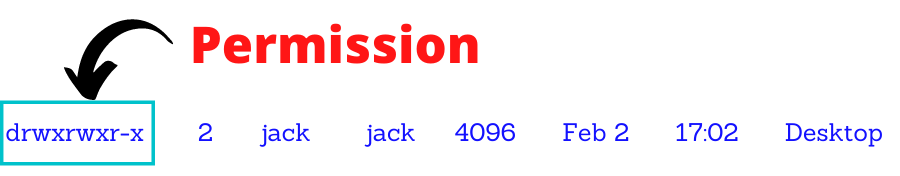
\includegraphics[scale=0.5]{content/chapter5/images/permission.png}
			\caption{"ls -l" output}
			\label{fig:Sample permission}
		\end{figure}
		
		Let's see this column in detail.
	\end{itemize}

	
	
	
\end{flushleft}

\newpage

